\documentclass[11pt]{article}
\usepackage[margin=0.7in]{geometry}
\usepackage{graphicx,booktabs,xcolor,hyperref}
\hypersetup{colorlinks=true,urlcolor=blue}
\setlength{\parindent}{0pt}\setlength{\parskip}{7pt}
\begin{document}
{\LARGE Pencil accounting: review snapshot}\\[4pt]
{\large Public synthetic known-answer mathematics}\\
29 October 2026, 19:10 UTC snapshot. Evidence-only report; no new cohort execution.

The existing plan-only aggregation input contains zero observed executions. It describes 1,260 workloads and retains null cost ratios in all 36 sensitivity cells. This count applies to the named input, not to historical experiments elsewhere. The observations below distinguish software validation, finite source review and future experimental admission.

\begin{center}\begin{tabular}{lr}\toprule
Plan-derived quantity [E1, E6] & Count\\\midrule
Workloads & 1,260\\
Measured candidate/reference pairs (5 streams per workload) & 6,300\\
Measured arm executions (candidate, rho, rho\_AA) & 18,900\\
Warmup arm executions (1 per arm and workload) & 3,780\\
Total expected execution slots & 22,680\\
Observed executions in this input & 0\\
Missing execution slots & 22,680\\\bottomrule\end{tabular}\end{center}
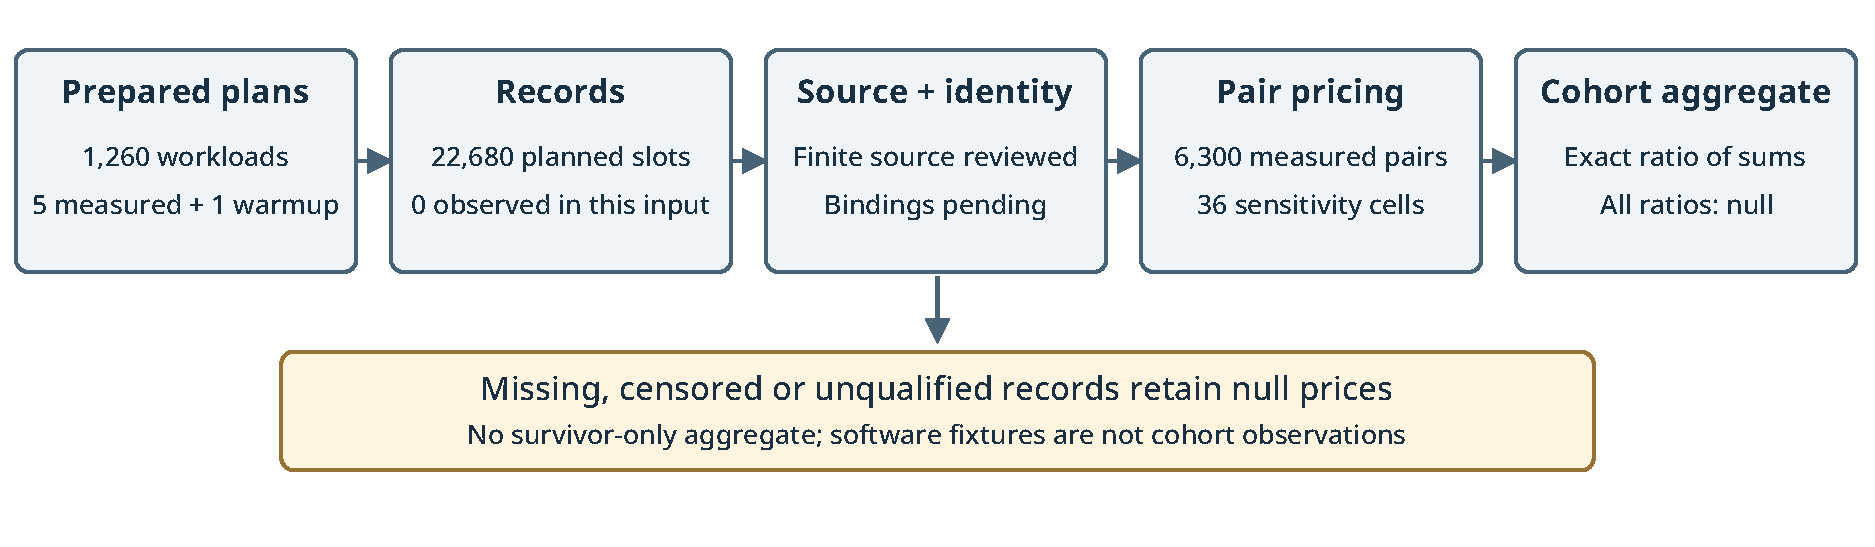
\includegraphics[width=\linewidth]{pipeline.pdf}

\textbf{Software validation.} The producer suite reports 49 passed, 0 failed and 1 ignored [E3]. The native analyzer reports 28 passed and 0 failed [E4]. The separately selected strict measurement test reports 1 passed and 49 filtered out [E5]. These are software tests, not sampled experimental targets. The full root release-library suite reports 5,277 passed, 0 failed and 123 ignored, with exit status 0. All 20 reviewed source files were unchanged after the run [E9].

\textbf{Aggregation rule.} The aggregate uses the ratio of exact sums over the prescribed cohort; missing or ineligible pairs prevent a qualified ratio. Each target's five measured rho\_AA/rho ratios must individually lie in the inclusive interval [0.90,1.10], separately for cold and online timing. This is an operational tolerance, not a confidence interval [E1].
\newpage
{\Large Source review and accounting boundary}

The finite source audit records \texttt{source\_review\_complete\_binding\_pending} [E2]. Its nine selected categories are field arithmetic; scalar arithmetic; outer and constructor validation; setup and transfer; collection, graph and elimination; hash and random generation; source verification; metadata cloning; and calibration. Each is recorded as covered under the declared finite model with no remaining listed uncovered site. This is a source-level review result, not a universal instruction census or an admitted experimental binary.

The finite algorithm model uses the inherited 36-cell sensitivity grid: square weight $S/M\in\{0,0.5,1\}$; inversion weight $I/M\in\{1,10,100,1000\}$; native-event weight $\{0,0.1,1\}$. Disjoint atomic scalar events, actual collection primitives, hash/random-generation events and copied metadata nodes follow the declared mapping. Diagnostic totals are not charged again [E1, E7].

Report formatting, serialization, allocation, RSS, wall and CPU time, parent verification, harness work, infrastructure and retries remain separately named resources. They are not assigned an invented conversion to field operations and are not assumed to cost zero. Calibration is retained separately and included once in the combined ratio [E1, E7]. No wall-time, memory or infrastructure measurements are presented here.

\textbf{Admission still pending at the source-audit snapshot.} An approved frozen protocol identifying policy and calibration treatment; exact instrument binary digest; reproducible build receipt binding the reviewed sources, Rust 1.99.1 and binary; an independent write-once coverage record satisfying the analyzer schema. The final root test and post-run source-hash checks have since passed [E9]. Remaining admission bindings are listed in the current audit [E2]. The audit's \texttt{reviewed\_complete\_emitted} and \texttt{cohort\_price\_ready} fields are both false. Prepared-plan integrity alone does not establish approval or authenticity.

\textbf{Evidence locations.} Paths below are relative to \texttt{research/pencil\_large\_prime\_20261029/}. Full SHA-256 digests and structured quantities are retained in \texttt{report.json}; generated-file hashes are in \texttt{SHA256SUMS}. The editable diagram is \texttt{pipeline.svg}, and this report's source is \texttt{report.tex}.
\begin{description}
\item[E1] {\footnotesize\path{validation/accounting/aggregate/actual-plan-only-summary-final.json}}
\item[E2] {\footnotesize\path{validation/accounting/finite-nine-category-source-audit.json}}
\item[E3] {\footnotesize\path{validation/accounting/consolidated-fixes/final-copy-producer-tests.log}}
\item[E4] {\footnotesize\path{validation/accounting/aggregate/integrated-tests.log}}
\item[E5] {\footnotesize\path{validation/accounting/consolidated-fixes/final-copy-exclusive-test.log}}
\item[E6] {\footnotesize\path{prepared_native_plans/result.json}}
\item[E7] {\footnotesize\path{validation/accounting/COST_BOUNDARY.md}}
\item[E8] {\footnotesize\path{validation/accounting/post-closure-root-release-lib-20261029T1855Z.source-manifest.json}}
\item[E9] {\footnotesize\path{validation/accounting/post-closure-root-release-lib-20261029T1855Z.source-hash-assertion.json}}
\end{description}\end{document}